\documentclass[twoside]{book}

% Packages required by doxygen
\usepackage{fixltx2e}
\usepackage{calc}
\usepackage{doxygen}
\usepackage[export]{adjustbox} % also loads graphicx
\usepackage{graphicx}
\usepackage[utf8]{inputenc}
\usepackage{makeidx}
\usepackage{multicol}
\usepackage{multirow}
\PassOptionsToPackage{warn}{textcomp}
\usepackage{textcomp}
\usepackage[nointegrals]{wasysym}
\usepackage[table]{xcolor}

% Font selection
\usepackage[T1]{fontenc}
\usepackage[scaled=.90]{helvet}
\usepackage{courier}
\usepackage{amssymb}
\usepackage{sectsty}
\renewcommand{\familydefault}{\sfdefault}
\allsectionsfont{%
  \fontseries{bc}\selectfont%
  \color{darkgray}%
}
\renewcommand{\DoxyLabelFont}{%
  \fontseries{bc}\selectfont%
  \color{darkgray}%
}
\newcommand{\+}{\discretionary{\mbox{\scriptsize$\hookleftarrow$}}{}{}}

% Page & text layout
\usepackage{geometry}
\geometry{%
  a4paper,%
  top=2.5cm,%
  bottom=2.5cm,%
  left=2.5cm,%
  right=2.5cm%
}
\tolerance=750
\hfuzz=15pt
\hbadness=750
\setlength{\emergencystretch}{15pt}
\setlength{\parindent}{0cm}
\setlength{\parskip}{3ex plus 2ex minus 2ex}
\makeatletter
\renewcommand{\paragraph}{%
  \@startsection{paragraph}{4}{0ex}{-1.0ex}{1.0ex}{%
    \normalfont\normalsize\bfseries\SS@parafont%
  }%
}
\renewcommand{\subparagraph}{%
  \@startsection{subparagraph}{5}{0ex}{-1.0ex}{1.0ex}{%
    \normalfont\normalsize\bfseries\SS@subparafont%
  }%
}
\makeatother

% Headers & footers
\usepackage{fancyhdr}
\pagestyle{fancyplain}
\fancyhead[LE]{\fancyplain{}{\bfseries\thepage}}
\fancyhead[CE]{\fancyplain{}{}}
\fancyhead[RE]{\fancyplain{}{\bfseries\leftmark}}
\fancyhead[LO]{\fancyplain{}{\bfseries\rightmark}}
\fancyhead[CO]{\fancyplain{}{}}
\fancyhead[RO]{\fancyplain{}{\bfseries\thepage}}
\fancyfoot[LE]{\fancyplain{}{}}
\fancyfoot[CE]{\fancyplain{}{}}
\fancyfoot[RE]{\fancyplain{}{\bfseries\scriptsize Generated by Doxygen }}
\fancyfoot[LO]{\fancyplain{}{\bfseries\scriptsize Generated by Doxygen }}
\fancyfoot[CO]{\fancyplain{}{}}
\fancyfoot[RO]{\fancyplain{}{}}
\renewcommand{\footrulewidth}{0.4pt}
\renewcommand{\chaptermark}[1]{%
  \markboth{#1}{}%
}
\renewcommand{\sectionmark}[1]{%
  \markright{\thesection\ #1}%
}

% Indices & bibliography
\usepackage{natbib}
\usepackage[titles]{tocloft}
\setcounter{tocdepth}{3}
\setcounter{secnumdepth}{5}
\makeindex

% Hyperlinks (required, but should be loaded last)
\usepackage{ifpdf}
\ifpdf
  \usepackage[pdftex,pagebackref=true]{hyperref}
\else
  \usepackage[ps2pdf,pagebackref=true]{hyperref}
\fi
\hypersetup{%
  colorlinks=true,%
  linkcolor=blue,%
  citecolor=blue,%
  unicode%
}

% Custom commands
\newcommand{\clearemptydoublepage}{%
  \newpage{\pagestyle{empty}\cleardoublepage}%
}

\usepackage{caption}
\captionsetup{labelsep=space,justification=centering,font={bf},singlelinecheck=off,skip=4pt,position=top}

%===== C O N T E N T S =====

\begin{document}

% Titlepage & ToC
\hypersetup{pageanchor=false,
             bookmarksnumbered=true,
             pdfencoding=unicode
            }
\pagenumbering{alph}
\begin{titlepage}
\vspace*{7cm}
\begin{center}%
{\Large Figura Geometrica \\[1ex]\large 0.\+001 }\\
\vspace*{1cm}
{\large Generated by Doxygen 1.8.13}\\
\end{center}
\end{titlepage}
\clearemptydoublepage
\pagenumbering{roman}
\tableofcontents
\clearemptydoublepage
\pagenumbering{arabic}
\hypersetup{pageanchor=true}

%--- Begin generated contents ---
\chapter{Hierarchical Index}
\section{Class Hierarchy}
This inheritance list is sorted roughly, but not completely, alphabetically\+:\begin{DoxyCompactList}
\item \contentsline{section}{Figura\+Geometrica}{\pageref{class_figura_geometrica}}{}
\begin{DoxyCompactList}
\item \contentsline{section}{Circulo}{\pageref{class_circulo}}{}
\item \contentsline{section}{Reta}{\pageref{class_reta}}{}
\item \contentsline{section}{Retangulo}{\pageref{class_retangulo}}{}
\end{DoxyCompactList}
\end{DoxyCompactList}

\chapter{Class Index}
\section{Class List}
Here are the classes, structs, unions and interfaces with brief descriptions\+:\begin{DoxyCompactList}
\item\contentsline{section}{\hyperlink{class_circulo}{Circulo} }{\pageref{class_circulo}}{}
\item\contentsline{section}{\hyperlink{class_figura_geometrica}{Figura\+Geometrica} }{\pageref{class_figura_geometrica}}{}
\item\contentsline{section}{\hyperlink{class_reta}{Reta} }{\pageref{class_reta}}{}
\item\contentsline{section}{\hyperlink{class_retangulo}{Retangulo} }{\pageref{class_retangulo}}{}
\end{DoxyCompactList}

\chapter{File Index}
\doxysection{File List}
Here is a list of all files with brief descriptions\+:\begin{DoxyCompactList}
\item\contentsline{section}{\mbox{\hyperlink{main_8cpp}{main.\+cpp}} }{\pageref{main_8cpp}}{}
\item\contentsline{section}{\mbox{\hyperlink{vetor2d_8cpp}{vetor2d.\+cpp}} }{\pageref{vetor2d_8cpp}}{}
\item\contentsline{section}{\mbox{\hyperlink{vetor2d_8h}{vetor2d.\+h}} }{\pageref{vetor2d_8h}}{}
\end{DoxyCompactList}

\chapter{Class Documentation}
\hypertarget{class_circulo}{}\section{Circulo Class Reference}
\label{class_circulo}\index{Circulo@{Circulo}}


{\ttfamily \#include $<$circulo.\+h$>$}



Inheritance diagram for Circulo\+:
\nopagebreak
\begin{figure}[H]
\begin{center}
\leavevmode
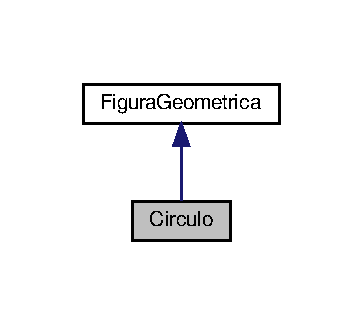
\includegraphics[width=174pt]{class_circulo__inherit__graph}
\end{center}
\end{figure}


Collaboration diagram for Circulo\+:
\nopagebreak
\begin{figure}[H]
\begin{center}
\leavevmode
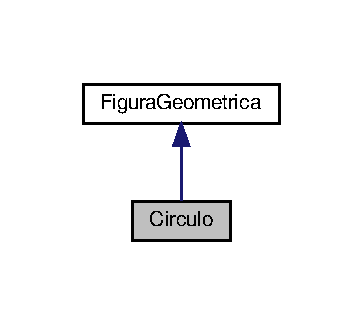
\includegraphics[width=174pt]{class_circulo__coll__graph}
\end{center}
\end{figure}
\subsection*{Public Member Functions}
\begin{DoxyCompactItemize}
\item 
\hyperlink{class_circulo_a6933bf908b78a4167684081a3a8f257f}{Circulo} ()
\item 
void \hyperlink{class_circulo_aa94899872fb6c586d1343df1d9ce0d86}{draw} ()
\end{DoxyCompactItemize}


\subsection{Constructor \& Destructor Documentation}
\mbox{\Hypertarget{class_circulo_a6933bf908b78a4167684081a3a8f257f}\label{class_circulo_a6933bf908b78a4167684081a3a8f257f}} 
\index{Circulo@{Circulo}!Circulo@{Circulo}}
\index{Circulo@{Circulo}!Circulo@{Circulo}}
\subsubsection{\texorpdfstring{Circulo()}{Circulo()}}
{\footnotesize\ttfamily Circulo\+::\+Circulo (\begin{DoxyParamCaption}{ }\end{DoxyParamCaption})}



\subsection{Member Function Documentation}
\mbox{\Hypertarget{class_circulo_aa94899872fb6c586d1343df1d9ce0d86}\label{class_circulo_aa94899872fb6c586d1343df1d9ce0d86}} 
\index{Circulo@{Circulo}!draw@{draw}}
\index{draw@{draw}!Circulo@{Circulo}}
\subsubsection{\texorpdfstring{draw()}{draw()}}
{\footnotesize\ttfamily void Circulo\+::draw (\begin{DoxyParamCaption}{ }\end{DoxyParamCaption})\hspace{0.3cm}{\ttfamily [virtual]}}



Reimplemented from \hyperlink{class_figura_geometrica_a417090ea2019fc1d58cdb345167aebea}{Figura\+Geometrica}.



The documentation for this class was generated from the following files\+:\begin{DoxyCompactItemize}
\item 
\hyperlink{circulo_8h}{circulo.\+h}\item 
\hyperlink{circulo_8cpp}{circulo.\+cpp}\end{DoxyCompactItemize}

\hypertarget{class_figura_geometrica}{}\section{Figura\+Geometrica Class Reference}
\label{class_figura_geometrica}\index{Figura\+Geometrica@{Figura\+Geometrica}}


A classe \hyperlink{class_figura_geometrica}{Figura\+Geometrica} serve como classe abstrata para criacao de outras figuras.  




{\ttfamily \#include $<$figurageometrica.\+h$>$}



Inheritance diagram for Figura\+Geometrica\+:\nopagebreak
\begin{figure}[H]
\begin{center}
\leavevmode
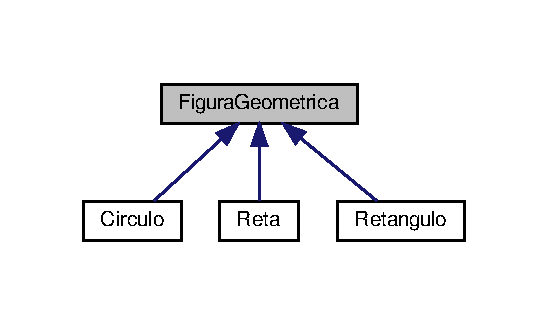
\includegraphics[width=263pt]{class_figura_geometrica__inherit__graph}
\end{center}
\end{figure}
\subsection*{Public Member Functions}
\begin{DoxyCompactItemize}
\item 
\hyperlink{class_figura_geometrica_a81d7c7efaea511e60a15f5a363138dd9}{Figura\+Geometrica} ()
\begin{DoxyCompactList}\small\item\em \hyperlink{class_figura_geometrica}{Figura\+Geometrica} eh o construtor da classe. \end{DoxyCompactList}\item 
virtual void \hyperlink{class_figura_geometrica_a727cea2befcb22b2457c088127fe041d}{draw} ()=0
\begin{DoxyCompactList}\small\item\em draw eh um metodo virtual puro que deve ser reimplementado nas classes derivadas \end{DoxyCompactList}\item 
virtual \hyperlink{class_figura_geometrica_ad13b9bccf1b14f6b9fbc662aad61ffd1}{$\sim$\+Figura\+Geometrica} ()
\begin{DoxyCompactList}\small\item\em $\sim$\+Figura\+Geometrica eh o destrutor virtual. Deve ser implementado para que os destrutores sejam chamados para cada uma das classes derivadas \end{DoxyCompactList}\end{DoxyCompactItemize}


\subsection{Detailed Description}
A classe \hyperlink{class_figura_geometrica}{Figura\+Geometrica} serve como classe abstrata para criacao de outras figuras. 

\hyperlink{class_figura_geometrica}{Figura\+Geometrica} implementa um conceito chamado de classe abstrata em C++. Permite que endereços de objetos de classes derivadas dela sejam armazenados em ponteiros dessa classe. 

\subsection{Constructor \& Destructor Documentation}
\mbox{\Hypertarget{class_figura_geometrica_a81d7c7efaea511e60a15f5a363138dd9}\label{class_figura_geometrica_a81d7c7efaea511e60a15f5a363138dd9}} 
\index{Figura\+Geometrica@{Figura\+Geometrica}!Figura\+Geometrica@{Figura\+Geometrica}}
\index{Figura\+Geometrica@{Figura\+Geometrica}!Figura\+Geometrica@{Figura\+Geometrica}}
\subsubsection{\texorpdfstring{Figura\+Geometrica()}{FiguraGeometrica()}}
{\footnotesize\ttfamily Figura\+Geometrica\+::\+Figura\+Geometrica (\begin{DoxyParamCaption}{ }\end{DoxyParamCaption})}



\hyperlink{class_figura_geometrica}{Figura\+Geometrica} eh o construtor da classe. 

\mbox{\Hypertarget{class_figura_geometrica_ad13b9bccf1b14f6b9fbc662aad61ffd1}\label{class_figura_geometrica_ad13b9bccf1b14f6b9fbc662aad61ffd1}} 
\index{Figura\+Geometrica@{Figura\+Geometrica}!````~Figura\+Geometrica@{$\sim$\+Figura\+Geometrica}}
\index{````~Figura\+Geometrica@{$\sim$\+Figura\+Geometrica}!Figura\+Geometrica@{Figura\+Geometrica}}
\subsubsection{\texorpdfstring{$\sim$\+Figura\+Geometrica()}{~FiguraGeometrica()}}
{\footnotesize\ttfamily Figura\+Geometrica\+::$\sim$\+Figura\+Geometrica (\begin{DoxyParamCaption}{ }\end{DoxyParamCaption})\hspace{0.3cm}{\ttfamily [virtual]}}



$\sim$\+Figura\+Geometrica eh o destrutor virtual. Deve ser implementado para que os destrutores sejam chamados para cada uma das classes derivadas 



\subsection{Member Function Documentation}
\mbox{\Hypertarget{class_figura_geometrica_a727cea2befcb22b2457c088127fe041d}\label{class_figura_geometrica_a727cea2befcb22b2457c088127fe041d}} 
\index{Figura\+Geometrica@{Figura\+Geometrica}!draw@{draw}}
\index{draw@{draw}!Figura\+Geometrica@{Figura\+Geometrica}}
\subsubsection{\texorpdfstring{draw()}{draw()}}
{\footnotesize\ttfamily virtual void Figura\+Geometrica\+::draw (\begin{DoxyParamCaption}{ }\end{DoxyParamCaption})\hspace{0.3cm}{\ttfamily [pure virtual]}}



draw eh um metodo virtual puro que deve ser reimplementado nas classes derivadas 



Implemented in \hyperlink{class_reta_a1c370279480f421bf617e5fbfbbb63a1}{Reta}, \hyperlink{class_circulo_aa94899872fb6c586d1343df1d9ce0d86}{Circulo}, and \hyperlink{class_retangulo_a48cb75fe7cd048727879c25485976444}{Retangulo}.



The documentation for this class was generated from the following files\+:\begin{DoxyCompactItemize}
\item 
\hyperlink{figurageometrica_8h}{figurageometrica.\+h}\item 
\hyperlink{figurageometrica_8cpp}{figurageometrica.\+cpp}\end{DoxyCompactItemize}

\hypertarget{class_reta}{}\section{Reta Class Reference}
\label{class_reta}\index{Reta@{Reta}}


{\ttfamily \#include $<$reta.\+h$>$}



Inheritance diagram for Reta\+:
\nopagebreak
\begin{figure}[H]
\begin{center}
\leavevmode
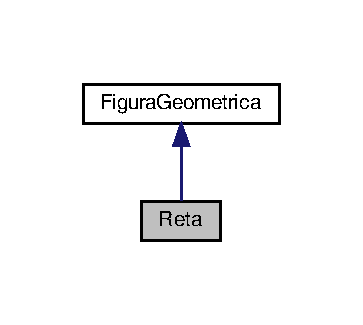
\includegraphics[width=174pt]{class_reta__inherit__graph}
\end{center}
\end{figure}


Collaboration diagram for Reta\+:
\nopagebreak
\begin{figure}[H]
\begin{center}
\leavevmode
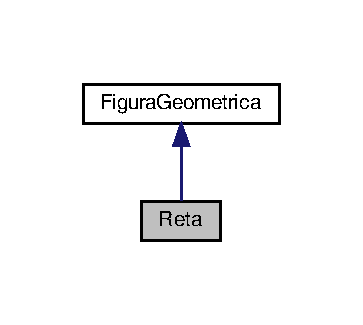
\includegraphics[width=174pt]{class_reta__coll__graph}
\end{center}
\end{figure}
\subsection*{Public Member Functions}
\begin{DoxyCompactItemize}
\item 
\hyperlink{class_reta_ab4754dffc985acd6cf4eec6f9bac668a}{Reta} ()
\item 
void \hyperlink{class_reta_a1c370279480f421bf617e5fbfbbb63a1}{draw} ()
\end{DoxyCompactItemize}


\subsection{Constructor \& Destructor Documentation}
\mbox{\Hypertarget{class_reta_ab4754dffc985acd6cf4eec6f9bac668a}\label{class_reta_ab4754dffc985acd6cf4eec6f9bac668a}} 
\index{Reta@{Reta}!Reta@{Reta}}
\index{Reta@{Reta}!Reta@{Reta}}
\subsubsection{\texorpdfstring{Reta()}{Reta()}}
{\footnotesize\ttfamily Reta\+::\+Reta (\begin{DoxyParamCaption}{ }\end{DoxyParamCaption})}



\subsection{Member Function Documentation}
\mbox{\Hypertarget{class_reta_a1c370279480f421bf617e5fbfbbb63a1}\label{class_reta_a1c370279480f421bf617e5fbfbbb63a1}} 
\index{Reta@{Reta}!draw@{draw}}
\index{draw@{draw}!Reta@{Reta}}
\subsubsection{\texorpdfstring{draw()}{draw()}}
{\footnotesize\ttfamily void Reta\+::draw (\begin{DoxyParamCaption}{ }\end{DoxyParamCaption})\hspace{0.3cm}{\ttfamily [virtual]}}



Reimplemented from \hyperlink{class_figura_geometrica_a417090ea2019fc1d58cdb345167aebea}{Figura\+Geometrica}.



The documentation for this class was generated from the following files\+:\begin{DoxyCompactItemize}
\item 
\hyperlink{reta_8h}{reta.\+h}\item 
\hyperlink{reta_8cpp}{reta.\+cpp}\end{DoxyCompactItemize}

\hypertarget{class_retangulo}{}\section{Retangulo Class Reference}
\label{class_retangulo}\index{Retangulo@{Retangulo}}


{\ttfamily \#include $<$retangulo.\+h$>$}



Inheritance diagram for Retangulo\+:
\nopagebreak
\begin{figure}[H]
\begin{center}
\leavevmode
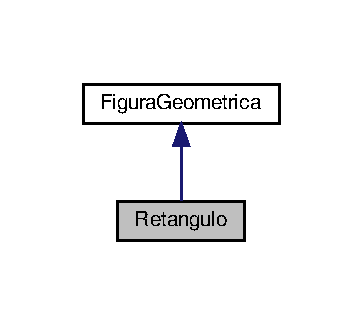
\includegraphics[width=174pt]{class_retangulo__inherit__graph}
\end{center}
\end{figure}


Collaboration diagram for Retangulo\+:
\nopagebreak
\begin{figure}[H]
\begin{center}
\leavevmode
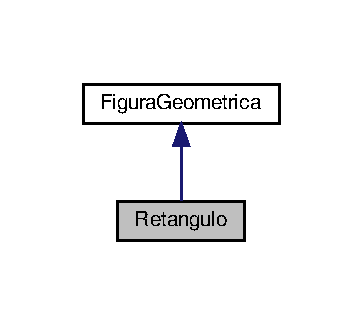
\includegraphics[width=174pt]{class_retangulo__coll__graph}
\end{center}
\end{figure}
\subsection*{Public Member Functions}
\begin{DoxyCompactItemize}
\item 
\hyperlink{class_retangulo_ac21a81cae046920c8bee401bcb879562}{Retangulo} ()
\item 
void \hyperlink{class_retangulo_a48cb75fe7cd048727879c25485976444}{draw} ()
\end{DoxyCompactItemize}


\subsection{Constructor \& Destructor Documentation}
\mbox{\Hypertarget{class_retangulo_ac21a81cae046920c8bee401bcb879562}\label{class_retangulo_ac21a81cae046920c8bee401bcb879562}} 
\index{Retangulo@{Retangulo}!Retangulo@{Retangulo}}
\index{Retangulo@{Retangulo}!Retangulo@{Retangulo}}
\subsubsection{\texorpdfstring{Retangulo()}{Retangulo()}}
{\footnotesize\ttfamily Retangulo\+::\+Retangulo (\begin{DoxyParamCaption}{ }\end{DoxyParamCaption})}



\subsection{Member Function Documentation}
\mbox{\Hypertarget{class_retangulo_a48cb75fe7cd048727879c25485976444}\label{class_retangulo_a48cb75fe7cd048727879c25485976444}} 
\index{Retangulo@{Retangulo}!draw@{draw}}
\index{draw@{draw}!Retangulo@{Retangulo}}
\subsubsection{\texorpdfstring{draw()}{draw()}}
{\footnotesize\ttfamily void Retangulo\+::draw (\begin{DoxyParamCaption}{ }\end{DoxyParamCaption})\hspace{0.3cm}{\ttfamily [virtual]}}



Reimplemented from \hyperlink{class_figura_geometrica_a417090ea2019fc1d58cdb345167aebea}{Figura\+Geometrica}.



The documentation for this class was generated from the following files\+:\begin{DoxyCompactItemize}
\item 
\hyperlink{retangulo_8h}{retangulo.\+h}\item 
\hyperlink{retangulo_8cpp}{retangulo.\+cpp}\end{DoxyCompactItemize}

\chapter{File Documentation}
\hypertarget{circulo_8cpp}{}\section{circulo.\+cpp File Reference}
\label{circulo_8cpp}\index{circulo.\+cpp@{circulo.\+cpp}}
{\ttfamily \#include \char`\"{}circulo.\+h\char`\"{}}\newline
{\ttfamily \#include $<$iostream$>$}\newline
Include dependency graph for circulo.\+cpp\+:
\nopagebreak
\begin{figure}[H]
\begin{center}
\leavevmode
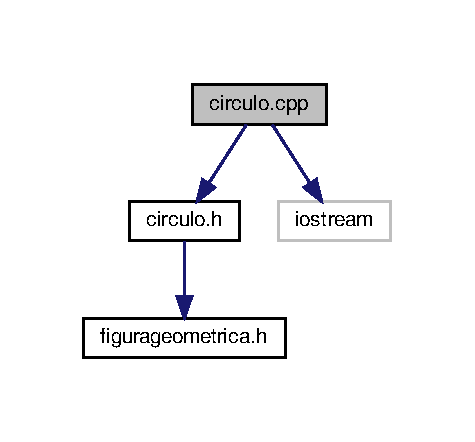
\includegraphics[width=228pt]{circulo_8cpp__incl}
\end{center}
\end{figure}

\hypertarget{circulo_8h}{}\section{circulo.\+h File Reference}
\label{circulo_8h}\index{circulo.\+h@{circulo.\+h}}
{\ttfamily \#include \char`\"{}figurageometrica.\+h\char`\"{}}\newline
Include dependency graph for circulo.\+h\+:
\nopagebreak
\begin{figure}[H]
\begin{center}
\leavevmode
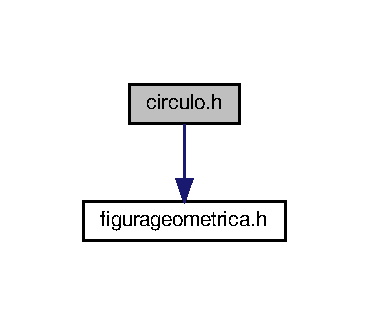
\includegraphics[width=177pt]{circulo_8h__incl}
\end{center}
\end{figure}
This graph shows which files directly or indirectly include this file\+:
\nopagebreak
\begin{figure}[H]
\begin{center}
\leavevmode
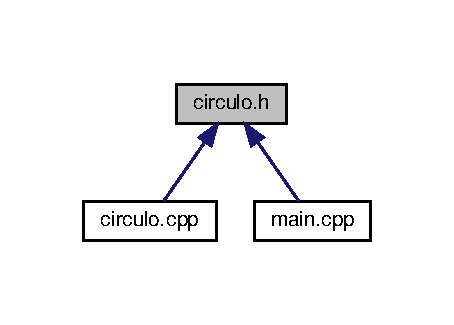
\includegraphics[width=218pt]{circulo_8h__dep__incl}
\end{center}
\end{figure}
\subsection*{Classes}
\begin{DoxyCompactItemize}
\item 
class \hyperlink{class_circulo}{Circulo}
\end{DoxyCompactItemize}

\hypertarget{figurageometrica_8cpp}{}\section{figurageometrica.\+cpp File Reference}
\label{figurageometrica_8cpp}\index{figurageometrica.\+cpp@{figurageometrica.\+cpp}}
{\ttfamily \#include \char`\"{}figurageometrica.\+h\char`\"{}}\newline
Include dependency graph for figurageometrica.\+cpp\+:
\nopagebreak
\begin{figure}[H]
\begin{center}
\leavevmode
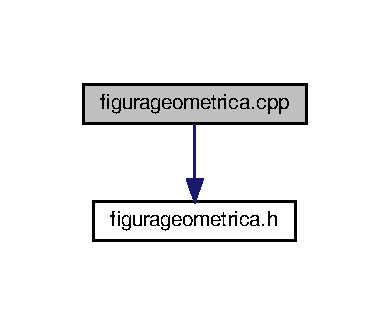
\includegraphics[width=187pt]{figurageometrica_8cpp__incl}
\end{center}
\end{figure}

\hypertarget{figurageometrica_8h}{}\section{figurageometrica.\+h File Reference}
\label{figurageometrica_8h}\index{figurageometrica.\+h@{figurageometrica.\+h}}
This graph shows which files directly or indirectly include this file\+:
\nopagebreak
\begin{figure}[H]
\begin{center}
\leavevmode
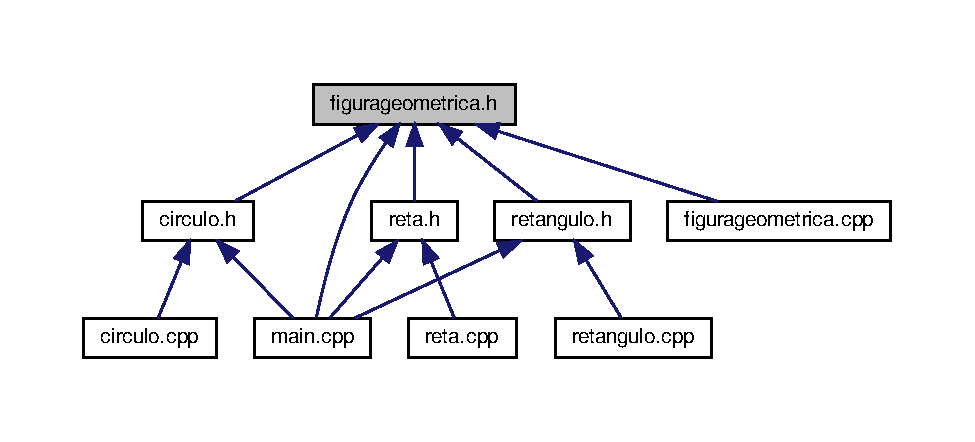
\includegraphics[width=350pt]{figurageometrica_8h__dep__incl}
\end{center}
\end{figure}
\subsection*{Classes}
\begin{DoxyCompactItemize}
\item 
class \hyperlink{class_figura_geometrica}{Figura\+Geometrica}
\end{DoxyCompactItemize}

\hypertarget{main_8cpp}{}\doxysection{main.\+cpp File Reference}
\label{main_8cpp}\index{main.cpp@{main.cpp}}
{\ttfamily \#include $<$iostream$>$}\newline
{\ttfamily \#include \char`\"{}motor.\+h\char`\"{}}\newline
Include dependency graph for main.\+cpp\+:
\nopagebreak
\begin{figure}[H]
\begin{center}
\leavevmode
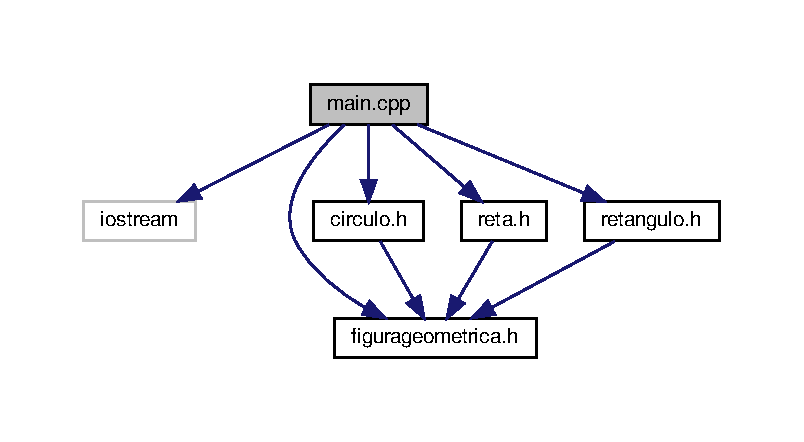
\includegraphics[width=230pt]{main_8cpp__incl}
\end{center}
\end{figure}
\doxysubsection*{Functions}
\begin{DoxyCompactItemize}
\item 
int \mbox{\hyperlink{main_8cpp_a840291bc02cba5474a4cb46a9b9566fe}{main}} (void)
\end{DoxyCompactItemize}


\doxysubsection{Function Documentation}
\mbox{\Hypertarget{main_8cpp_a840291bc02cba5474a4cb46a9b9566fe}\label{main_8cpp_a840291bc02cba5474a4cb46a9b9566fe}} 
\index{main.cpp@{main.cpp}!main@{main}}
\index{main@{main}!main.cpp@{main.cpp}}
\doxysubsubsection{\texorpdfstring{main()}{main()}}
{\footnotesize\ttfamily int main (\begin{DoxyParamCaption}\item[{void}]{ }\end{DoxyParamCaption})}


\hypertarget{reta_8cpp}{}\section{reta.\+cpp File Reference}
\label{reta_8cpp}\index{reta.\+cpp@{reta.\+cpp}}
{\ttfamily \#include \char`\"{}reta.\+h\char`\"{}}\newline
{\ttfamily \#include $<$iostream$>$}\newline
Include dependency graph for reta.\+cpp\+:
\nopagebreak
\begin{figure}[H]
\begin{center}
\leavevmode
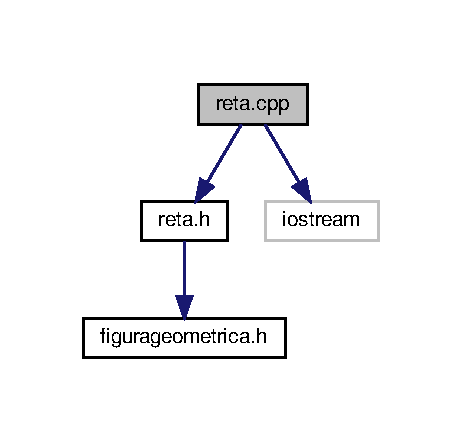
\includegraphics[width=222pt]{reta_8cpp__incl}
\end{center}
\end{figure}

\hypertarget{reta_8h}{}\section{reta.\+h File Reference}
\label{reta_8h}\index{reta.\+h@{reta.\+h}}
{\ttfamily \#include \char`\"{}figurageometrica.\+h\char`\"{}}\newline
Include dependency graph for reta.\+h\+:\nopagebreak
\begin{figure}[H]
\begin{center}
\leavevmode
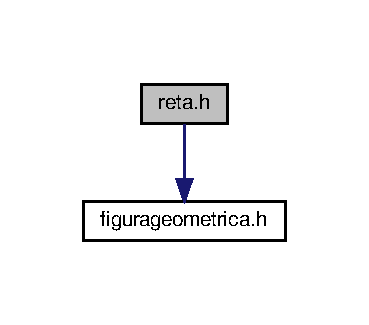
\includegraphics[width=177pt]{reta_8h__incl}
\end{center}
\end{figure}
This graph shows which files directly or indirectly include this file\+:\nopagebreak
\begin{figure}[H]
\begin{center}
\leavevmode
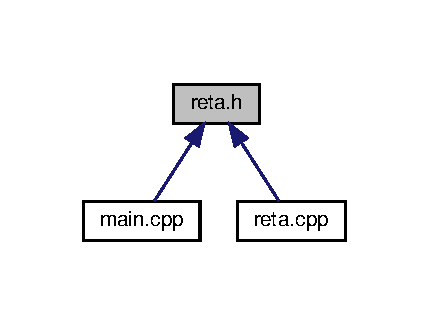
\includegraphics[width=206pt]{reta_8h__dep__incl}
\end{center}
\end{figure}
\subsection*{Classes}
\begin{DoxyCompactItemize}
\item 
class \hyperlink{class_reta}{Reta}
\begin{DoxyCompactList}\small\item\em A classe reta implementa uma reta no plano cartesiano. \end{DoxyCompactList}\end{DoxyCompactItemize}

\hypertarget{retangulo_8cpp}{}\section{retangulo.\+cpp File Reference}
\label{retangulo_8cpp}\index{retangulo.\+cpp@{retangulo.\+cpp}}
{\ttfamily \#include \char`\"{}retangulo.\+h\char`\"{}}\newline
{\ttfamily \#include $<$iostream$>$}\newline
Include dependency graph for retangulo.\+cpp\+:
\nopagebreak
\begin{figure}[H]
\begin{center}
\leavevmode
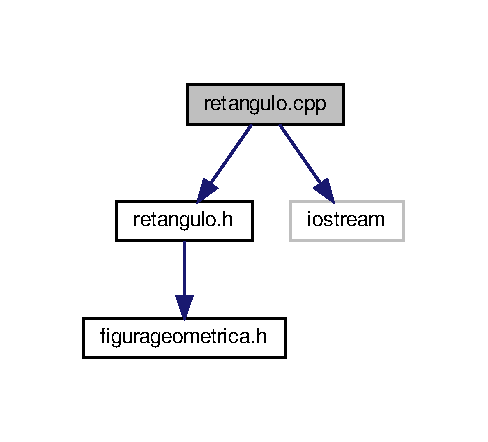
\includegraphics[width=234pt]{retangulo_8cpp__incl}
\end{center}
\end{figure}

\hypertarget{retangulo_8h}{}\section{retangulo.\+h File Reference}
\label{retangulo_8h}\index{retangulo.\+h@{retangulo.\+h}}
{\ttfamily \#include \char`\"{}figurageometrica.\+h\char`\"{}}\newline
Include dependency graph for retangulo.\+h\+:\nopagebreak
\begin{figure}[H]
\begin{center}
\leavevmode
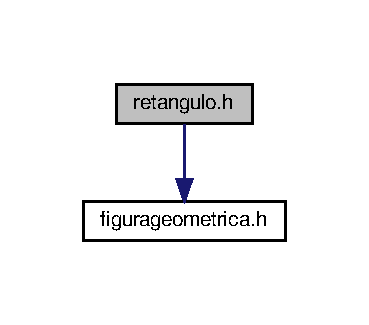
\includegraphics[width=177pt]{retangulo_8h__incl}
\end{center}
\end{figure}
This graph shows which files directly or indirectly include this file\+:\nopagebreak
\begin{figure}[H]
\begin{center}
\leavevmode
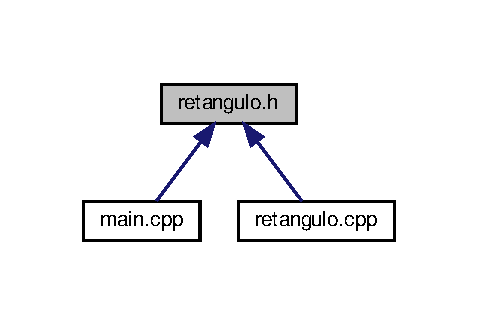
\includegraphics[width=230pt]{retangulo_8h__dep__incl}
\end{center}
\end{figure}
\subsection*{Classes}
\begin{DoxyCompactItemize}
\item 
class \hyperlink{class_retangulo}{Retangulo}
\end{DoxyCompactItemize}

%--- End generated contents ---

% Index
\backmatter
\newpage
\phantomsection
\clearemptydoublepage
\addcontentsline{toc}{chapter}{Index}
\printindex

\end{document}
